% Wyrd III GUI tutorial. Build: make (Tectonic). Screenshots: images/ (gt-*.png), regenerated from real
% runs by shots/make_gui_shots.py.
\documentclass[11pt]{article}
\usepackage[OT1]{fontenc}
\usepackage{mathptmx}
\usepackage[scaled=.90]{helvet}
\usepackage{courier}
\usepackage[letterpaper,margin=1.1in,top=1.0in,bottom=1.0in]{geometry}
\usepackage{graphicx,xcolor,fancyhdr,titlesec,caption,enumitem,fancyvrb,listings,float,url}
\usepackage[colorlinks=true,linkcolor=blue!60!black,urlcolor=blue!60!black,citecolor=blue!60!black,bookmarksopen=true,bookmarksnumbered=true,pdfborder={0 0 0}]{hyperref}

\definecolor{banner}{HTML}{1F5FBF}
\definecolor{codebg}{HTML}{F4F4F4}
\definecolor{cmt}{HTML}{2E7D32}

\titleformat{\section}{\sffamily\Large\bfseries}{\thesection}{0.8em}{}
\titleformat{\subsection}{\sffamily\large\bfseries}{\thesubsection}{0.8em}{}
\titlespacing*{\section}{0pt}{16pt}{8pt}
\titlespacing*{\subsection}{0pt}{12pt}{5pt}

\pagestyle{fancy}
\fancyhf{}
\lhead{\scriptsize\textsc{Wyrd III GUI Tutorial: Doing Everything in the Interface}}
\rhead{\scriptsize\textit{For Wyrd III 0.1}}
\lfoot{\small Yggdrasil III}
\rfoot{\small\thepage}
\renewcommand{\headrulewidth}{0.3pt}
\renewcommand{\footrulewidth}{0pt}

\setlength{\parindent}{0pt}
\setlength{\parskip}{6pt}
\captionsetup{font=small,labelfont=bf,labelsep=period}
\setlist[enumerate]{leftmargin=2.2em,itemsep=4pt,topsep=2pt}
\setlist[itemize]{itemsep=2pt,topsep=2pt}

% UI labels and commands
\newcommand{\ui}[1]{\textsf{#1}}
\newcommand{\menu}[1]{\textsf{#1}}
\newcommand{\cmd}[1]{\texttt{#1}}
\newcommand{\gt}{\,$>$\,}

% Pasted real output (transcripts/*.txt are written by shots/make_shots.py)
\DefineVerbatimEnvironment{Out}{Verbatim}{fontsize=\footnotesize,frame=single,rulecolor=\color{gray},
  framesep=3pt,baselinestretch=0.95}
\newcommand{\transcript}[1]{{\VerbatimInput[fontsize=\footnotesize,frame=single,rulecolor=\color{gray},
  framesep=3pt]{transcripts/#1.txt}}}
\newcommand{\widetranscript}[1]{{\VerbatimInput[fontsize=\scriptsize,frame=single,rulecolor=\color{gray},
  framesep=3pt]{transcripts/#1.txt}}}

\lstset{basicstyle=\ttfamily\footnotesize,backgroundcolor=\color{codebg},frame=single,
  rulecolor=\color{gray},keywordstyle=\bfseries,commentstyle=\color{cmt}\itshape,columns=fullflexible,
  keepspaces=true,showstringspaces=false,breaklines=true,xleftmargin=0pt}
\lstdefinelanguage{Verilog}{morekeywords={module,endmodule,input,output,wire,reg,always,posedge,
  if,else,begin,end,assign,parameter},sensitive=true,morecomment=[l]{//},morecomment=[s]{/*}{*/}}
\lstdefinelanguage{TOMLx}{morekeywords={},morecomment=[l]{\#},morestring=[b]"}

\newcommand{\shot}[3][1.0]{\begin{figure}[H]\centering
  \includegraphics[width=#1\linewidth]{images/#2.png}\caption{#3}\label{fig:#2}\end{figure}}

\newcommand{\note}[1]{\par\smallskip\noindent\fbox{\parbox{0.94\linewidth}{\small\textbf{Note.} #1}}\par\smallskip}

\begin{document}

\begin{center}
{\sffamily\LARGE Wyrd III GUI Tutorial\\[2pt] Doing Everything in the Interface}
\end{center}
\vspace{2pt}
\noindent\colorbox{banner}{\parbox{\dimexpr\linewidth-2\fboxsep}{\color{white}\sffamily\itshape\small For Wyrd III 0.1\quad(Yggdrasil III suite)\hfill October 2026}}

\begingroup\hypersetup{linkcolor=blue!60!black}
\renewcommand{\contentsname}{Contents}
\tableofcontents
\endgroup
\clearpage

\section{Introduction}

This tutorial walks through Wyrd III with the mouse. You open the graphical interface, create a project, describe
your machine, run a design through Odin III and VPR, read the results and the messages, compare two versions of the
design, simulate it cycle by cycle, look at the sample project, and play a level of Midgard III. Every step of Wyrd III
itself is done in the interface and has a numbered figure. The command-line tutorial (\cmd{wyrd-tutorial.pdf}) covers the same
tool from the terminal.

Doing this tutorial, the reader will learn about:
\begin{itemize}
\item Starting the interface and finding the project tree, the tabs and the Messages and Flow docks
\item Creating a project, adding a design and editing \cmd{wyrd.toml} with live validation
\item Setting the machine settings (tools, memory budget, VPR for the floorplan) in the Settings dialog
\item Running the flow, reading the Flow log, the run tree, the results table and the Messages dock
\item Comparing two projects
\item Simulating a design with Bifrost III and viewing its waveform
\item The sample project and Midgard III (Verilog Town): placing sensors, editing the Verilog, starting a level
\end{itemize}

Every picture comes from a real run on one machine: a script (\cmd{docs/tutorial-gui/shots/make\_gui\_shots.py}) drives the
real windows with Qt's offscreen platform and grabs each widget, so the tutorial can be regenerated after a change.
The Midgard III pictures are grabs of the game's own drawing surface. The numbers are those of the real runs. In the pictures
the project folder is a scratch folder; yours will have the name you choose.

\textbf{Conventions.} Menu entries are written \menu{Menu1 \gt Menu2 \gt Item}. Buttons and fields are in sans-serif,
\ui{like this}. File and folder housekeeping (making folders, copying files, editing Verilog in an editor) is done in a terminal,
and those commands are shown after a \cmd{\$} prompt; everything Wyrd III does is done in the interface.

\subsection{What you need}

Wyrd III runs on Linux, including WSL on Windows (WSLg shows the windows). You need Python 3.11 or later, a built
Odin III (the programs \cmd{odin3} and \cmd{odin3-flow}), a VTR checkout for \cmd{vpr} and the architecture files, and Wyrd III
installed with its interface, simulation and game extras:
\begin{lstlisting}[language={}]
$ python3 -m venv .venv
$ .venv/bin/pip install -e ".[gui,sim,midgard]"
\end{lstlisting}
The machine settings go in \cmd{\textasciitilde/.config/wyrd/machine.toml}. If the file does not exist, \cmd{wyrd config init} writes
one with the tools it finds, and Section~\ref{sec:settings} shows how to check and change the values in the interface.
The design used here is the small \cmd{counteradd} project of the command-line tutorial: a 4-bit counter plus a 4-bit adder with a step
input. Its Verilog sources are in \cmd{docs/tutorial/project/src} of the Wyrd III repository.

\section{Starting Wyrd III}

\begin{enumerate}
\item Start the interface with \cmd{wyrd-gui} (it takes an optional project folder, and without one it reopens the last project).
\begin{lstlisting}[language={}]
$ wyrd-gui
\end{lstlisting}
\item The main window opens (Figure~\ref{fig:gt-start}). The \ui{Project} dock on the left will show the designs, recipes and architectures of
a project. The centre has four tabs: \ui{Source}, \ui{Report}, \ui{wyrd.toml} and \ui{Simulate}; they are grey until a project is open.
The bottom has two tabbed docks, \ui{Messages} and \ui{Flow}. The \menu{View} menu shows or hides the docks.
\end{enumerate}

\shot[0.95]{gt-start}{The Wyrd III main window with no project open.}

\section{Creating a Project}

\subsection{The folder and the sources}

Wyrd III creates the project file, but the folder and the Verilog files come from you. In a terminal, make a folder and copy the three source
files into a \cmd{src} folder in it:
\begin{lstlisting}[language={}]
$ mkdir -p ~/wyrd-gui-demo
$ cp -r docs/tutorial/project/src ~/wyrd-gui-demo/src
\end{lstlisting}

\subsection{New Project}

\begin{enumerate}
\item Open the \menu{File} menu (Figure~\ref{fig:gt-menu-file}). \menu{New Project...} asks for a folder; \menu{Open Project...} (Ctrl+O) opens an
existing one; \menu{Recent} lists the last projects.
\item Choose \menu{File \gt New Project...} and pick \cmd{wyrd-gui-demo}. Wyrd III writes a commented \cmd{wyrd.toml} into it and opens it.
The template names a placeholder file, \cmd{CHANGE\_ME.v}, so it does not validate yet. The \ui{wyrd.toml} tab shows the line that is wrong in red
and the message under the text (Figure~\ref{fig:gt-new-project}); only this tab is enabled until the file is valid.
\end{enumerate}

\begin{figure}[H]\centering
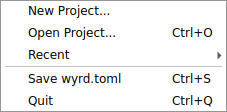
\includegraphics[width=0.30\linewidth]{images/gt-menu-file.png}
\caption{The \menu{File} menu.}\label{fig:gt-menu-file}
\end{figure}

\shot[0.95]{gt-new-project}{The new project: the template does not validate until the placeholder design is replaced.}

\subsection{Add the design}

\begin{enumerate}
\item Open \menu{Project \gt Add design...} (Figure~\ref{fig:gt-menu-project}). The dialog has a name, a list of files, the top module and the box
\ui{Add to [sweep] design}.
\item Name the design \cmd{counteradd}, add \cmd{src/add4.v}, \cmd{src/counter.v} and \cmd{src/top.v} with \ui{Add files...}, set the top module to
\cmd{top} and tick the box (Figure~\ref{fig:gt-adddesign}). Press \ui{OK}.
\item The dialog appends a \cmd{[[design]]} block to the text in the \ui{wyrd.toml} tab and adds the name to the sweep. Nothing is saved yet
(Figure~\ref{fig:gt-added}).
\end{enumerate}

\begin{figure}[H]\centering
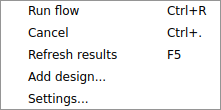
\includegraphics[width=0.30\linewidth]{images/gt-menu-project.png}
\caption{The \menu{Project} menu.}\label{fig:gt-menu-project}
\end{figure}

\begin{figure}[H]\centering
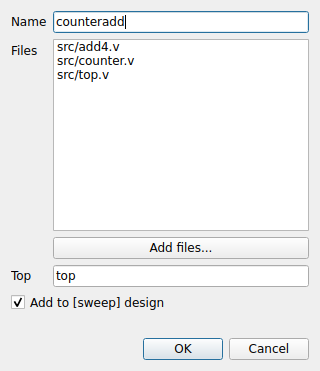
\includegraphics[width=0.55\linewidth]{images/gt-adddesign.png}
\caption{The Add design dialog, filled in.}\label{fig:gt-adddesign}
\end{figure}

\shot[0.95]{gt-added}{The new design is in the editor text. The placeholder design is still there and the file is still invalid.}

\subsection{Edit wyrd.toml and save}

The \ui{wyrd.toml} tab is an ordinary text editor with a validation line under it: a valid file shows how many runs it expands to.
Edit the text in the tab: delete the placeholder \cmd{[[design]]} block and its comment, change the project name to \cmd{counteradd},
and add a second architecture, \cmd{"EArch"}, to the \cmd{arch} list of \cmd{[sweep]}. The line under the text turns green and says
\ui{Valid: 2 runs} (Figure~\ref{fig:gt-edited}). Press \ui{Save} (Ctrl+S). The project reloads: the tree shows the design with its
three files, the recipe and the two architectures, and the other tabs are enabled. Double-click a file in the tree to see it in the
\ui{Source} tab (Figure~\ref{fig:gt-source}).

\shot[0.95]{gt-edited}{The edited \cmd{wyrd.toml}: valid, two runs. The Add design block is at the end of the text.}
\shot[0.95]{gt-source}{The \ui{Source} tab with \cmd{src/top.v}. The tree on the left shows the saved project.}

\section{Project Settings}\label{sec:settings}

Machine settings describe your computer, not the experiment, so they are not in \cmd{wyrd.toml}. Choose
\menu{Project \gt Settings...} (Figure~\ref{fig:gt-settings}). The top line is the file being edited. The dialog has three groups:

\begin{itemize}
\item \ui{tools}: the \cmd{odin3} and \cmd{odin3-flow} programs, \ui{vtr\_root} (the VTR checkout, for \cmd{vpr}, \cmd{abc} and the architecture files) and
\ui{vpr\_gui} (a VPR built with graphics; the Floorplan button of Section~\ref{sec:floorplan} uses it).
\item \ui{resources}: \ui{mem\_budget} (the share of memory Wyrd III may use), \ui{jobs} (parallel runs), \ui{launcher} (\cmd{systemd} runs each step in a
memory-limited scope) and the free-disk check.
\item \ui{defaults}: the memory a VPR or other step is first given, the factor by which a remembered peak is raised, the factor applied after a
memory kill, and the step timeout in seconds.
\end{itemize}

Press \ui{OK} to save or \ui{Cancel}; a value that does not parse is reported in the dialog and the file is not written.

\begin{figure}[H]\centering
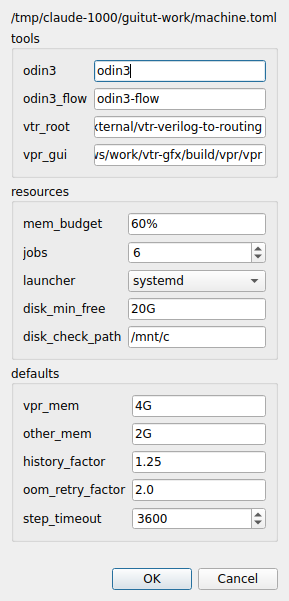
\includegraphics[width=0.38\linewidth]{images/gt-settings.png}
\caption{The Settings dialog. The values are those of the machine this tutorial was made on.}\label{fig:gt-settings}
\end{figure}

\section{Running the Flow}

\begin{enumerate}
\item Click the \ui{Flow} dock (Figure~\ref{fig:gt-flow-idle}). \ui{Jobs} and \ui{Memory budget} override the machine settings for this run when set;
\ui{Force} runs again the runs that are already \cmd{ok}.
\item Press \ui{Run} (or \menu{Project \gt Run flow}, Ctrl+R). The bar counts finished runs and the log lists each run as it ends
(Figure~\ref{fig:gt-running}). \ui{Cancel} (Ctrl+.) stops the running steps; finished runs stay.
\item When the bar reaches 100\% the status line reads \ui{all runs ok} (Figure~\ref{fig:gt-flow-done}). The Report tab is filled in.
\end{enumerate}

The Flow dock runs \cmd{wyrd run} as a program, so what you see is what the command line does. Both runs of this project take
about a second each.

\shot[0.95]{gt-flow-idle}{The Flow dock before the first run.}
\shot[0.95]{gt-running}{A run in progress.}
\shot[0.95]{gt-flow-done}{Both runs finished. The Report tab lists one node for each run.}

\section{Results}

\subsection{The run tree and the Summary}

The tree in the \ui{Report} tab has \ui{All runs} first, one node for each run (design and architecture) and \ui{Compare} last.
Expand \ui{counteradd / EArch} and select \ui{Summary} (Figure~\ref{fig:gt-summary}): the status, the LUTs and CLBs, the hard blocks
(\ui{memory} and \ui{mult\_36}), Fmax in MHz (1000 divided by the critical path), the minimum channel width, the critical path in ns, the
run directory and the run key. For the EArch run: 4 LUTs, 2 CLBs, a critical path of 2.565 ns (Fmax 389.8 MHz) and a channel
width of 20.

\shot[0.95]{gt-summary}{The Summary of the EArch run.}

\subsection{All runs}

Select \ui{All runs} (Figure~\ref{fig:gt-allruns}) for the table that \cmd{wyrd table} prints, one row for each run. Here both
architectures give 4 LUTs and 2 CLBs; the critical path is 2.565 ns on EArch and 1.984 ns on the K6 architecture.

\shot[0.95]{gt-allruns}{All runs of the project in one table.}

\subsection{Log nodes and the Messages dock}

Each step has a node with its log files. Expand \ui{Step 0: odin3-flow} and select a log: the page shows the file
(Figure~\ref{fig:gt-log}). Switch to the \ui{Messages} dock: it lists the warnings and errors that Wyrd III parsed from the logs of the
selected run, with the tool that wrote them, the text and the file and line.

\begin{enumerate}
\item Use the drop-down at the top of the dock to show \ui{All}, \ui{Errors} or \ui{Warnings}. Here five warnings come from VPR.
\item Double-click a row. The \ui{Source} tab opens the file at that line, with the line highlighted (Figure~\ref{fig:gt-messages-source}).
\end{enumerate}

\shot[0.95]{gt-log}{A log node of the first step.}
\shot[0.95]{gt-messages-source}{The Messages dock filtered to warnings; a double-click opened the VPR log at the warning.}

\section{Comparing Two Projects}

We compare the design with a variant whose output is registered. Make a copy of the project folder without its results and put the
registered \cmd{top.v} into it:
\begin{lstlisting}[language={}]
$ mkdir -p ~/wyrd-gui-demo2
$ cp -r ~/wyrd-gui-demo/src ~/wyrd-gui-demo/wyrd.toml ~/wyrd-gui-demo2/
$ cp docs/tutorial/project/variants/top_registered.v ~/wyrd-gui-demo2/src/top.v
\end{lstlisting}

\begin{enumerate}
\item Choose \menu{File \gt Open Project...} and open \cmd{wyrd-gui-demo2}, then press \ui{Run} in the Flow dock.
\item In the \ui{Report} tab select \ui{Compare} (Figure~\ref{fig:gt-compare-empty}) and press \ui{Compare with project...}. Choose
\cmd{wyrd-gui-demo}.
\item The table lists, for every run of both projects, each metric of the open project (A) and the chosen one (B) and the ratio B/A
(Figure~\ref{fig:gt-compare}). The registered design has the shorter critical path on EArch: 2.078 ns against 2.565 ns, a ratio of
1.234; LUTs, CLBs and channel width are unchanged. Runs found in only one project are listed under the table.
\end{enumerate}

\shot[0.95]{gt-compare-empty}{The Compare page of the project with the registered output.}
\shot[0.95]{gt-compare}{The comparison with the first project.}

\section{Simulation with Bifrost III}

The \ui{Simulate} tab (Tools menu, Ctrl+T) runs the design cycle by cycle with Odin III's simulator. Re-open \cmd{wyrd-gui-demo}
and select the tab (Figure~\ref{fig:gt-sim-tab}).

\begin{enumerate}
\item Choose the design and, if the design has more than one top, the top module. Press \ui{Compile}. The panel lists the signals
(Figure~\ref{fig:gt-sim-compiled}): name, width and kind (input, output or internal).
\item Type values into the input cells: \cmd{rst} = 1 and press \ui{Step} for one clock cycle, then \cmd{rst} = 0, \cmd{step} = 9 and \ui{Step N}
for five cycles. The output \cmd{total} counts up by the step each cycle (Figure~\ref{fig:gt-sim-stepped}).
\item Change \cmd{step} to 3 and run ten more cycles. The \ui{Waveform} tab draws every signal with its values (Figure~\ref{fig:gt-sim-waveform}):
the reset pulse, the step input and \cmd{total} in hexadecimal.
\item \ui{Run}, \ui{Reset}, \ui{Run random} and \ui{Run vectors} are the other ways to drive the design. \ui{Save VCD...} writes the waveform,
\ui{Save vectors...} the stimulus, and \ui{Open in GTKWave} opens the VCD if GTKWave is installed.
\end{enumerate}

\shot[0.95]{gt-sim-tab}{The Simulate tab before compiling.}
\shot[0.95]{gt-sim-compiled}{Compiled: the signals of the design.}
\shot[0.95]{gt-sim-stepped}{After reset and five cycles with \cmd{step} = 9.}
\shot[0.95]{gt-sim-waveform}{The waveform view after ten more cycles with \cmd{step} = 3.}

\section{The Floorplan}\label{sec:floorplan}

The \ui{Floorplan} button in the \ui{Report} tab (next to the tree) shows the placement and routing of the selected run in VPR's
own graphics window. It re-runs VPR with graphics for that run, using the VPR named by \ui{vpr\_gui} in the Settings dialog
(Section~\ref{sec:settings}); if \ui{vpr\_gui} is empty it uses the VPR named in the run's log. The button is disabled, with the reason as its tooltip,
when no VPR can be used. Wyrd III needs a VPR built with Qt6 graphics for this; the manual's Floorplan setup section describes how to build one.
The Flow log prints the command it starts. The window is VPR's, not Wyrd III's, and it is not shown in a figure here because it is drawn
with OpenGL, which cannot be captured by the scripted screenshots used in this tutorial.

\section{The Sample Project and Midgard III}

\subsection{The sample project}

The repository's \cmd{samples} folder is a project with three designs: \cmd{single} (a LUT-only design), \cmd{multi} (several files in folders)
and \cmd{dsp} (a memory and a multiplier), run on both architectures. Open it with \menu{File \gt Open Project...} (Figure~\ref{fig:gt-samples-open}),
press \ui{Run}, and select \ui{All runs} (Figure~\ref{fig:gt-samples}): six runs, \cmd{dsp} using one memory and one multiplier block.

\shot[0.95]{gt-samples-open}{The sample project opened; the tree shows its three designs.}
\shot[0.95]{gt-samples}{The sample project after \ui{Run}: six runs.}

\subsection{Midgard III (Verilog Town)}

Midgard III is a game inside Wyrd III, a close replication of verilogTown. You write one Verilog module for each traffic light of a
small town, and cars drive through it. The modules are simulated by Odin III through Bifrost III; one tick is one clock edge of
your module, 60 ticks a second at speed 1.

\subsubsection*{Starting the game}

The game has three entry points: \menu{Tools \gt Midgard III (Verilog Town)} in Wyrd III (Figure~\ref{fig:gt-menu-tools}), the command \cmd{midgard}
(which also takes \cmd{--level N}, 0 to 12, and \cmd{--data-dir}), and the level editor, \menu{Tools \gt Midgard III Level Editor} or
\cmd{midgard-editor}. The game needs pygame; without it the first menu entry is greyed with a tooltip that says why.

\begin{figure}[H]\centering
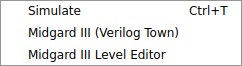
\includegraphics[width=0.40\linewidth]{images/gt-menu-tools.png}
\caption{The \menu{Tools} menu.}\label{fig:gt-menu-tools}
\end{figure}

The main menu lists levels 1 to 12, the tutorial level (level 0), the high scores and the credits. Choose level 1
(Figure~\ref{fig:gt-mg-menu}). The game creates the files you own in its data directory (\cmd{\$MIDGARD\_HOME} or
\cmd{\textasciitilde/.local/share/midgard}): \cmd{Lv1/VerilogFiles/Traffic\_signal\_set\_0.v} and one file for each other intersection,
from a starter module.

\begin{figure}[H]\centering
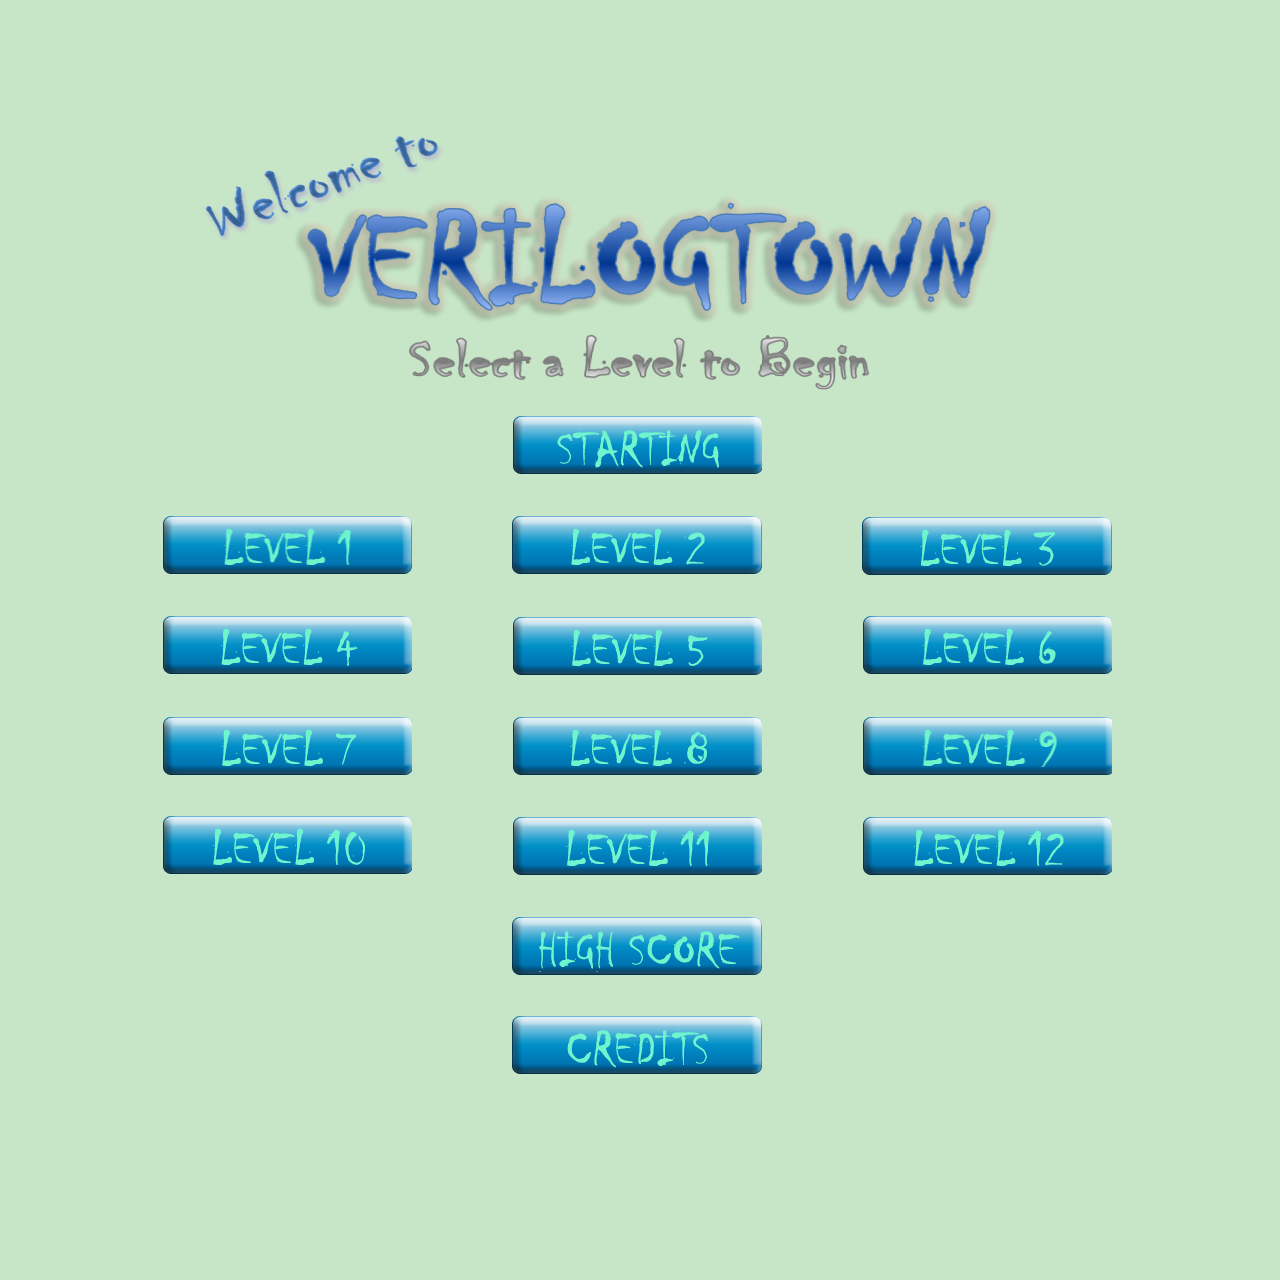
\includegraphics[width=0.46\linewidth]{images/gt-mg-menu.png}\hfill
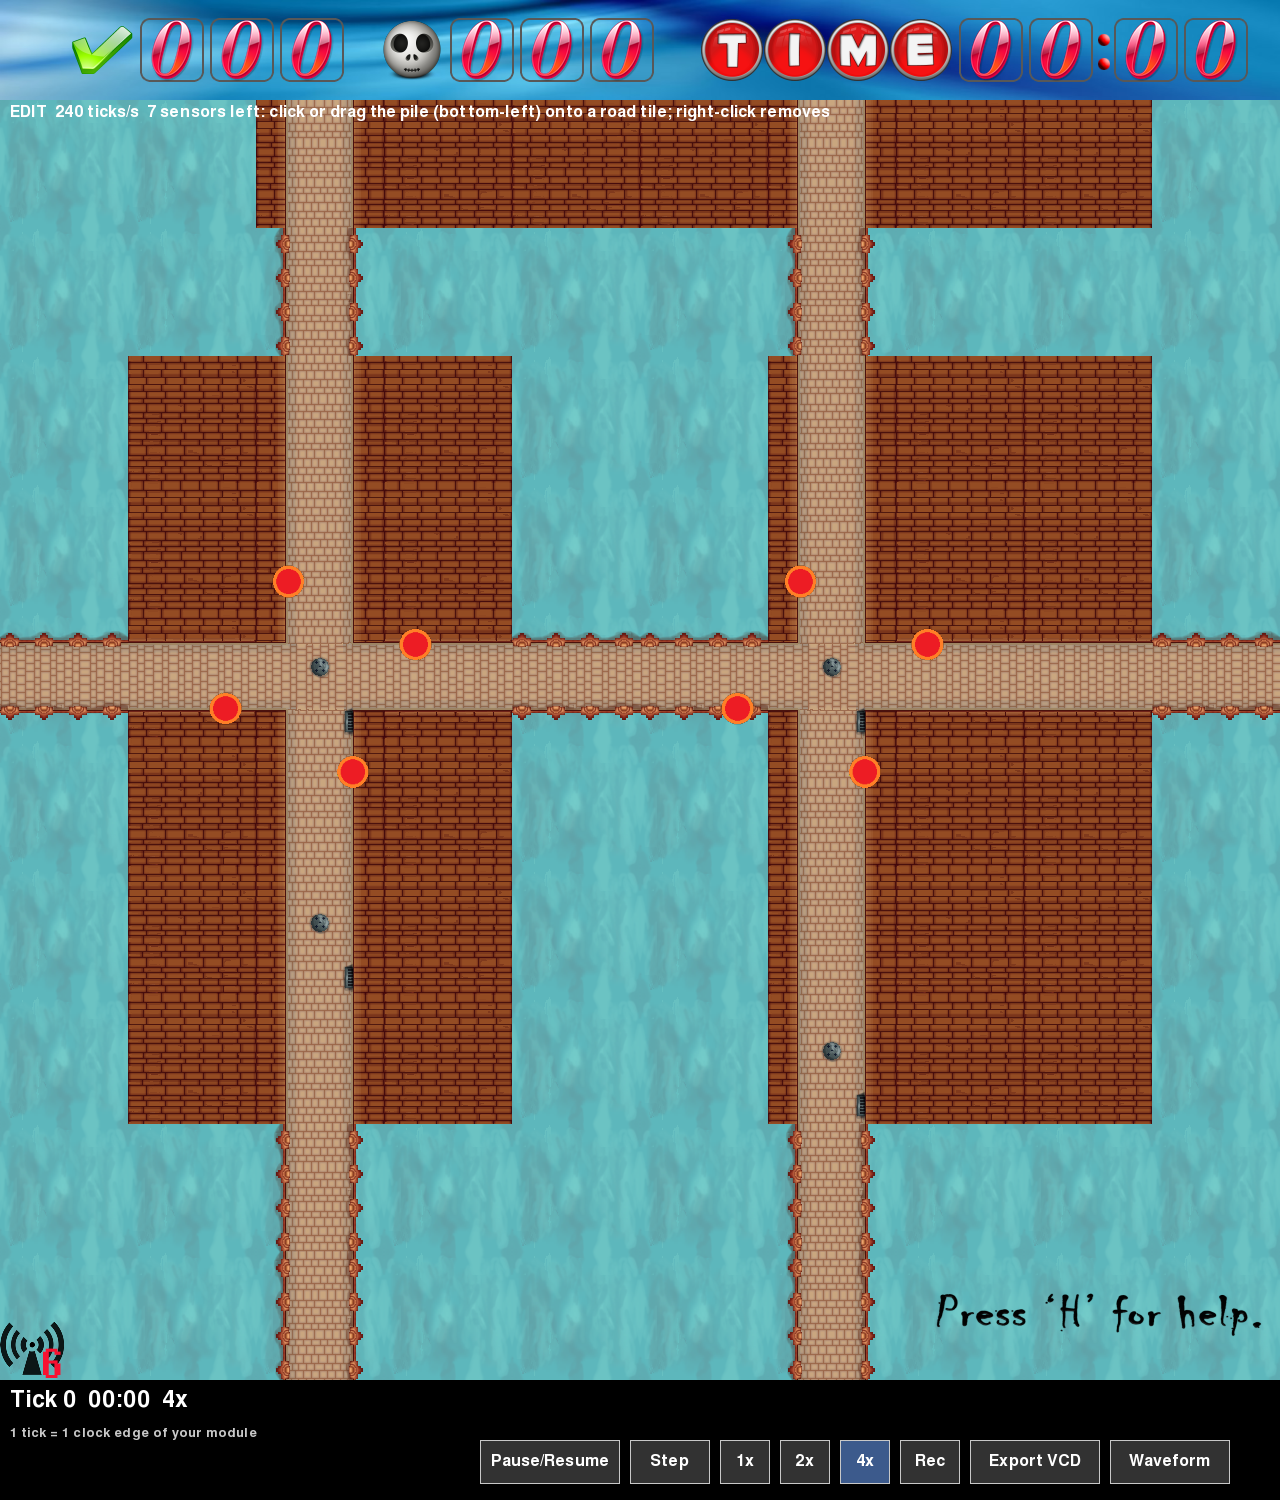
\includegraphics[width=0.46\linewidth]{images/gt-mg-level-edit.png}
\caption{The main menu (left) and level 1 in the edit phase (right). The sensor pile, with the number of sensors left, is at the bottom-left of the map.}\label{fig:gt-mg-menu}
\end{figure}

\subsubsection*{The help overlay (H)}

Press \ui{H} in the edit phase or when the level is paused. The help overlay lists the keys (Figure~\ref{fig:gt-mg-help}); press \ui{H} again to close it.
The overlay shows S (start), P (pause), M (main menu), R (restart), = and - (zoom in and out), the four arrow keys (move the map), C (clear
sensors) and H (help). The game also reacts to the keys listed in Table~\ref{tab:keys}, which the overlay does not show.

\begin{figure}[H]\centering
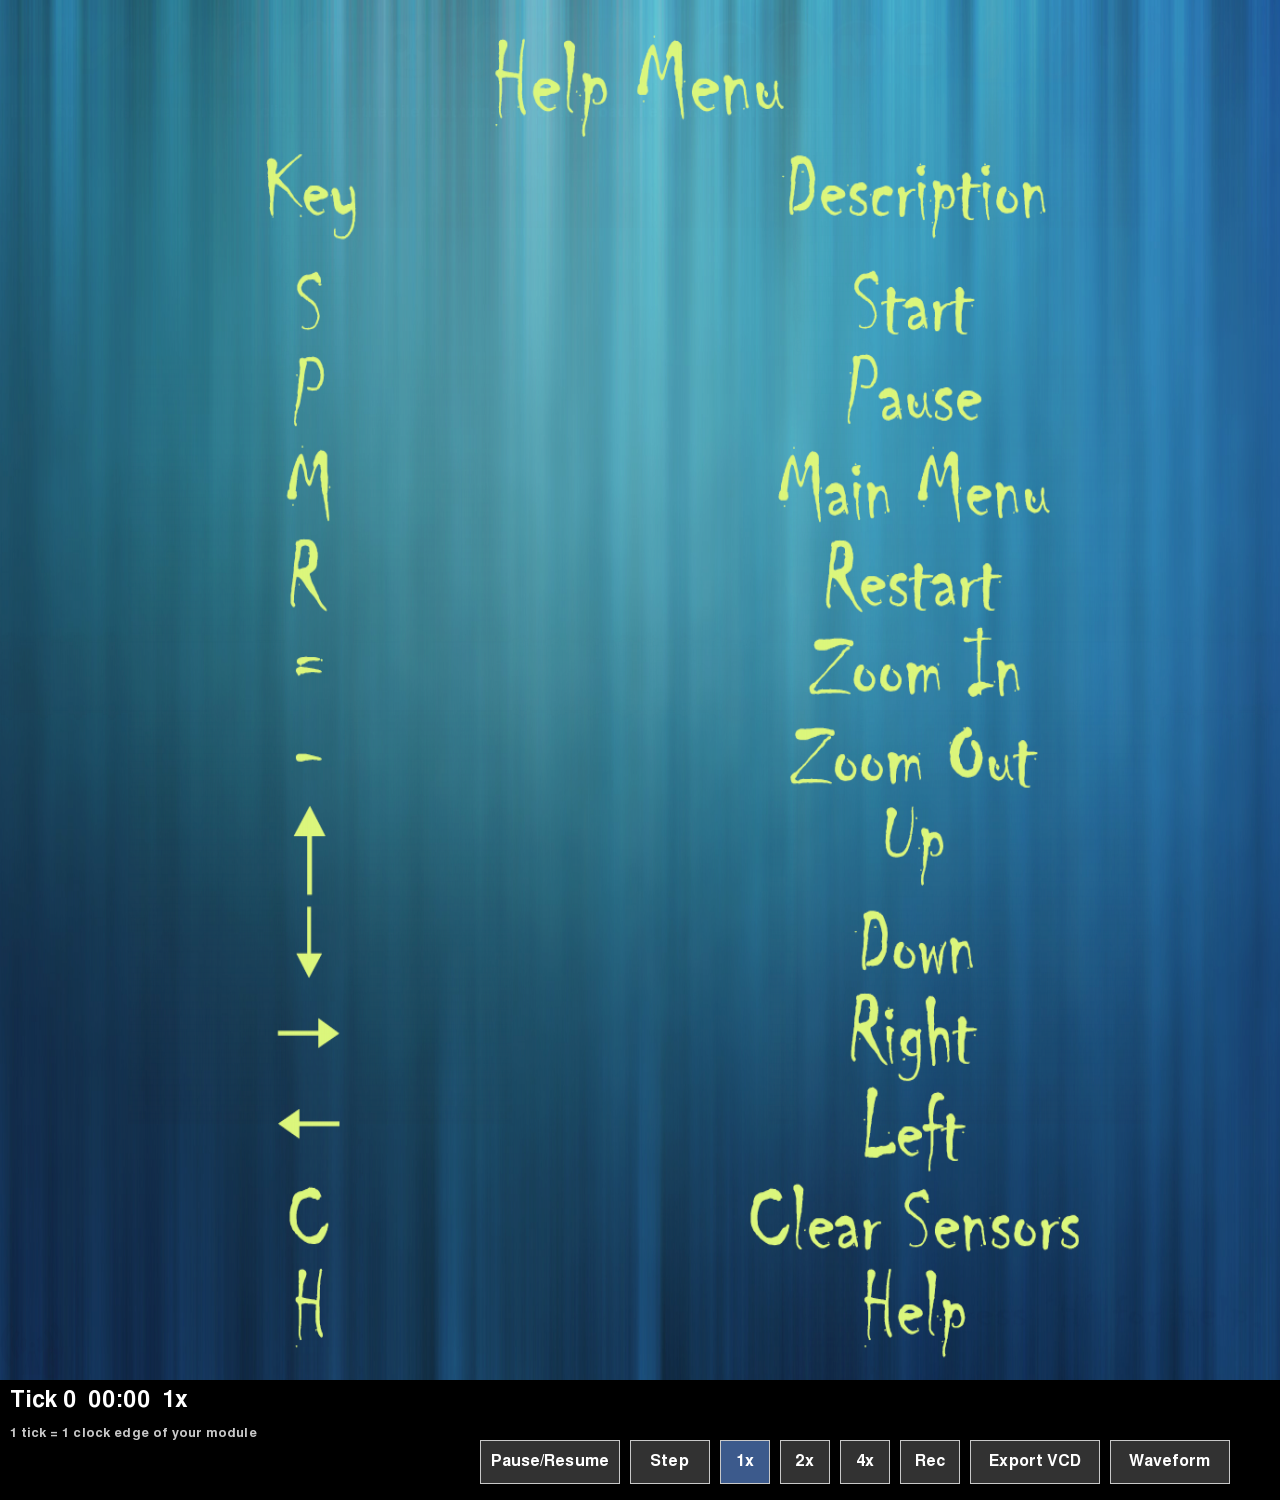
\includegraphics[width=0.46\linewidth]{images/gt-mg-help.png}
\caption{The help overlay of Midgard III.}\label{fig:gt-mg-help}
\end{figure}

\begin{table}[H]\centering\small
\begin{tabular}{ll}
\textbf{Key} & \textbf{Action}\\\hline
\ui{S} & start the level (edit phase), or resume (paused)\\
\ui{P} or \ui{X} & pause (running)\\
\ui{.} (period) & step one tick (starts paused in the edit phase)\\
\ui{1}, \ui{2}, \ui{4} & speed 1x, 2x, 4x\\
\ui{V} & arm or stop recording\\
\ui{E} & export a VCD of each recorded intersection (paused or finished)\\
\ui{R} & restart the level\\
\ui{M} & main menu (edit phase)\\
\ui{C} & remove all sensors (edit phase)\\
\ui{H} & help overlay (edit phase or paused)\\
\ui{Q} or \ui{=}; \ui{A} or \ui{-} & zoom in; zoom out\\
arrow keys & move the map\\
\end{tabular}
\caption{The keys of the level screen, as the code binds them.}\label{tab:keys}
\end{table}

\subsubsection*{Placing and dragging a sensor}

A level has seven general sensors, numbered 0 to 6. A sensor on a road tile tells your Verilog whether a car is on that tile and where it
is going. Sensors can only be placed in the edit phase.

\begin{enumerate}
\item Click the sensor pile at the bottom-left of the map: the highest-numbered unplaced sensor follows the mouse
(Figure~\ref{fig:gt-mg-sensor-in-hand}). Click a road tile that is not part of an intersection to place it
(Figure~\ref{fig:gt-mg-sensor-placed}). The sensor file is saved at once.
\item To move it, press on the placed sensor, drag it to another road tile and release (Figure~\ref{fig:gt-mg-drag}). Right-click removes a sensor; \ui{C} removes all.
\end{enumerate}

\begin{figure}[H]\centering
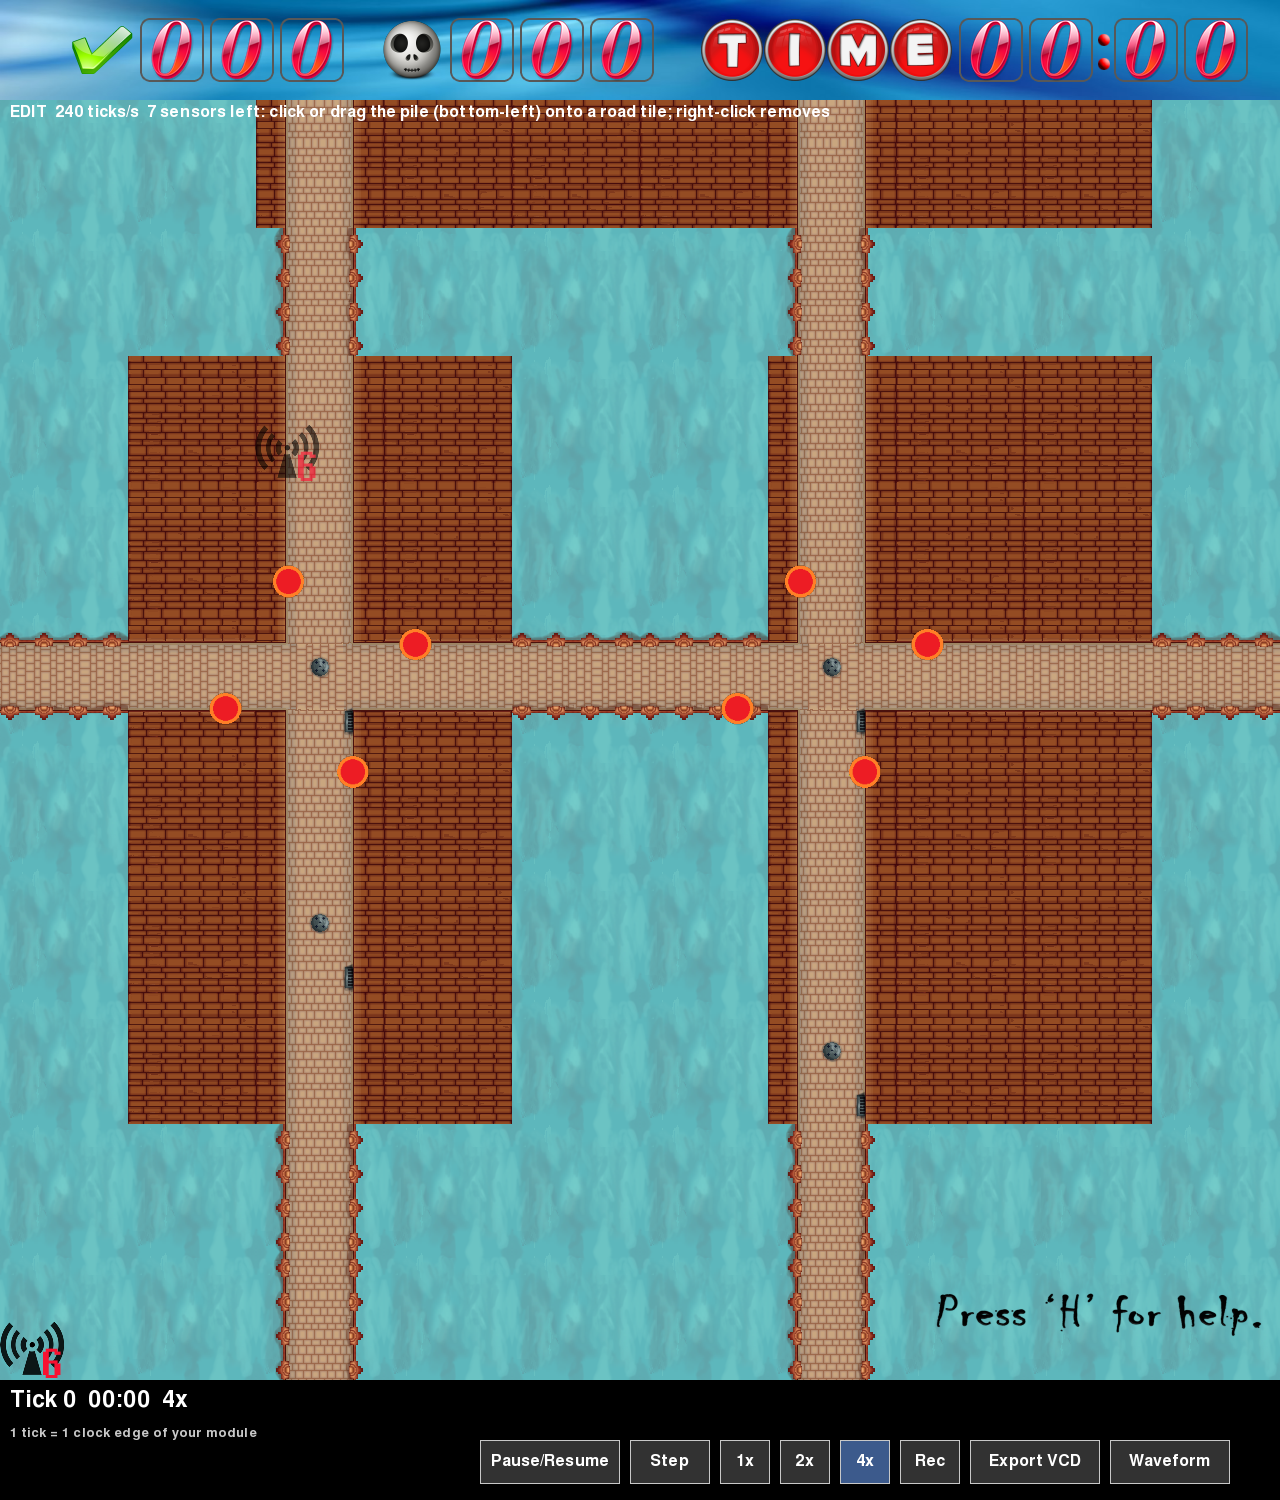
\includegraphics[width=0.46\linewidth]{images/gt-mg-sensor-in-hand.png}\hfill
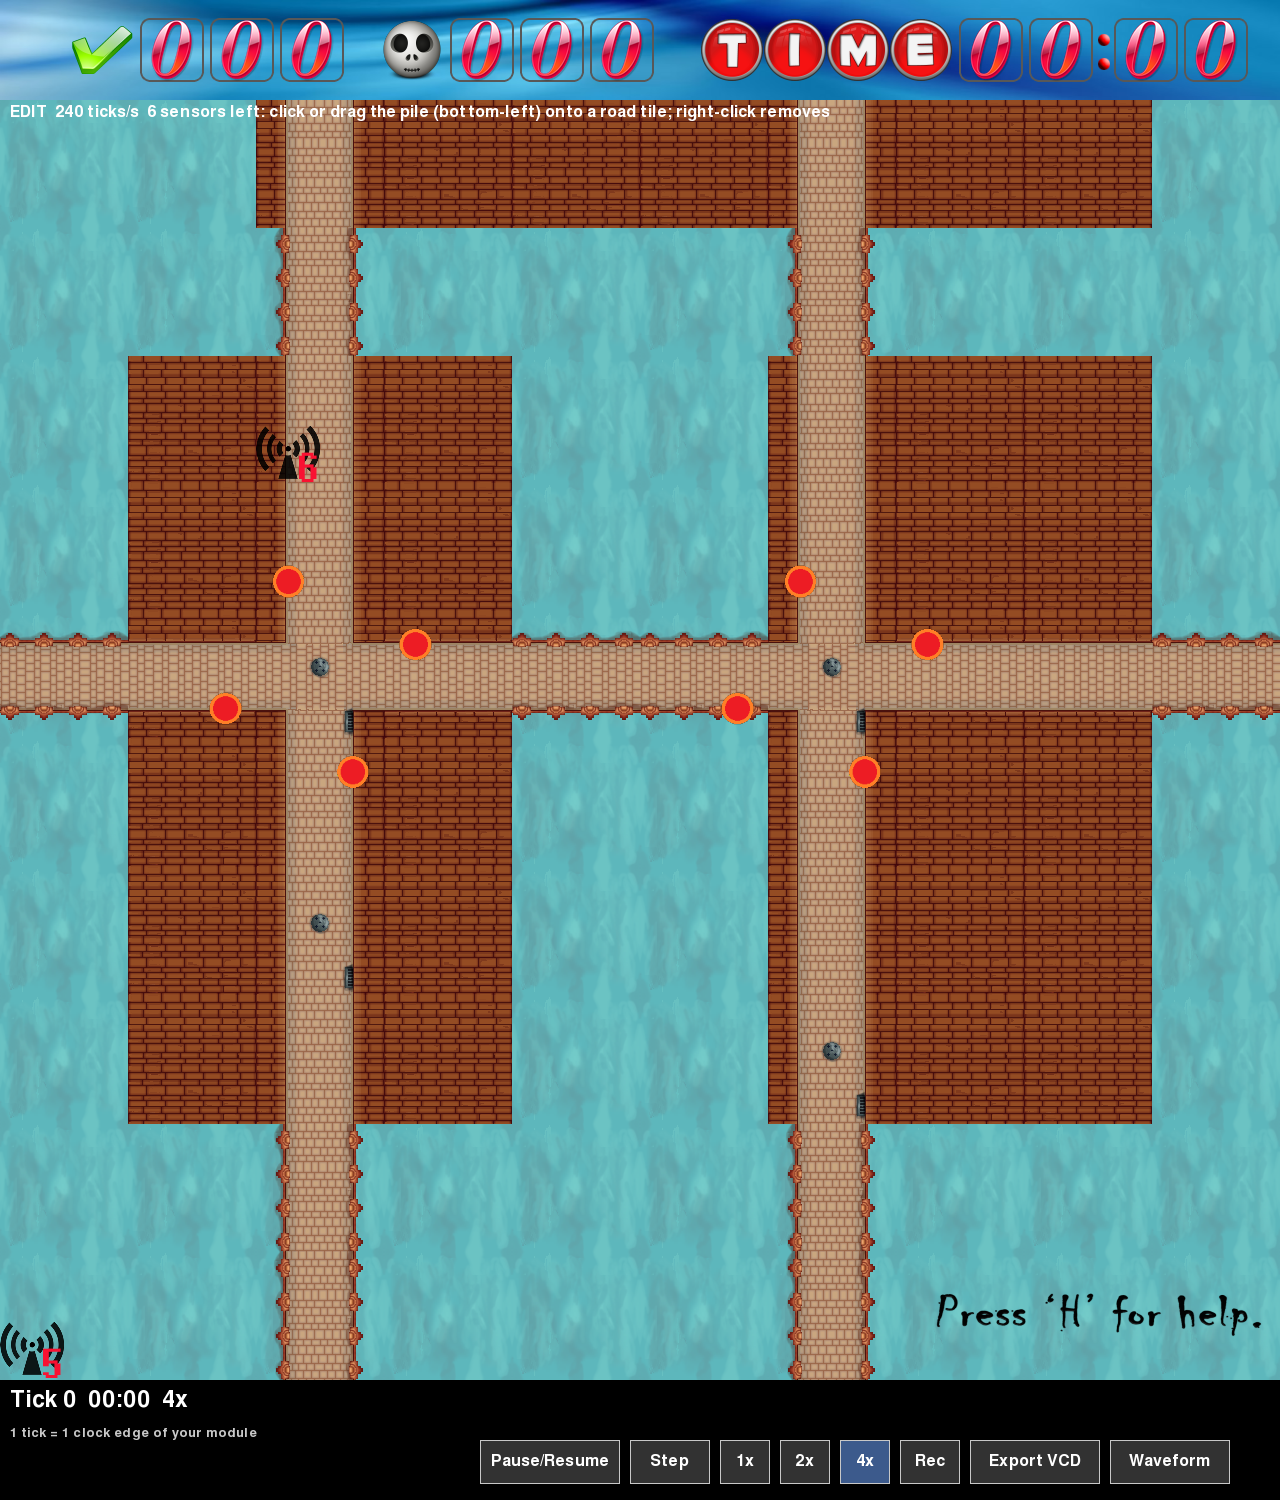
\includegraphics[width=0.46\linewidth]{images/gt-mg-sensor-placed.png}
\caption{Sensor 6 in the hand, and placed on a road tile.}\label{fig:gt-mg-sensor-in-hand}\label{fig:gt-mg-sensor-placed}
\end{figure}

\begin{figure}[H]\centering
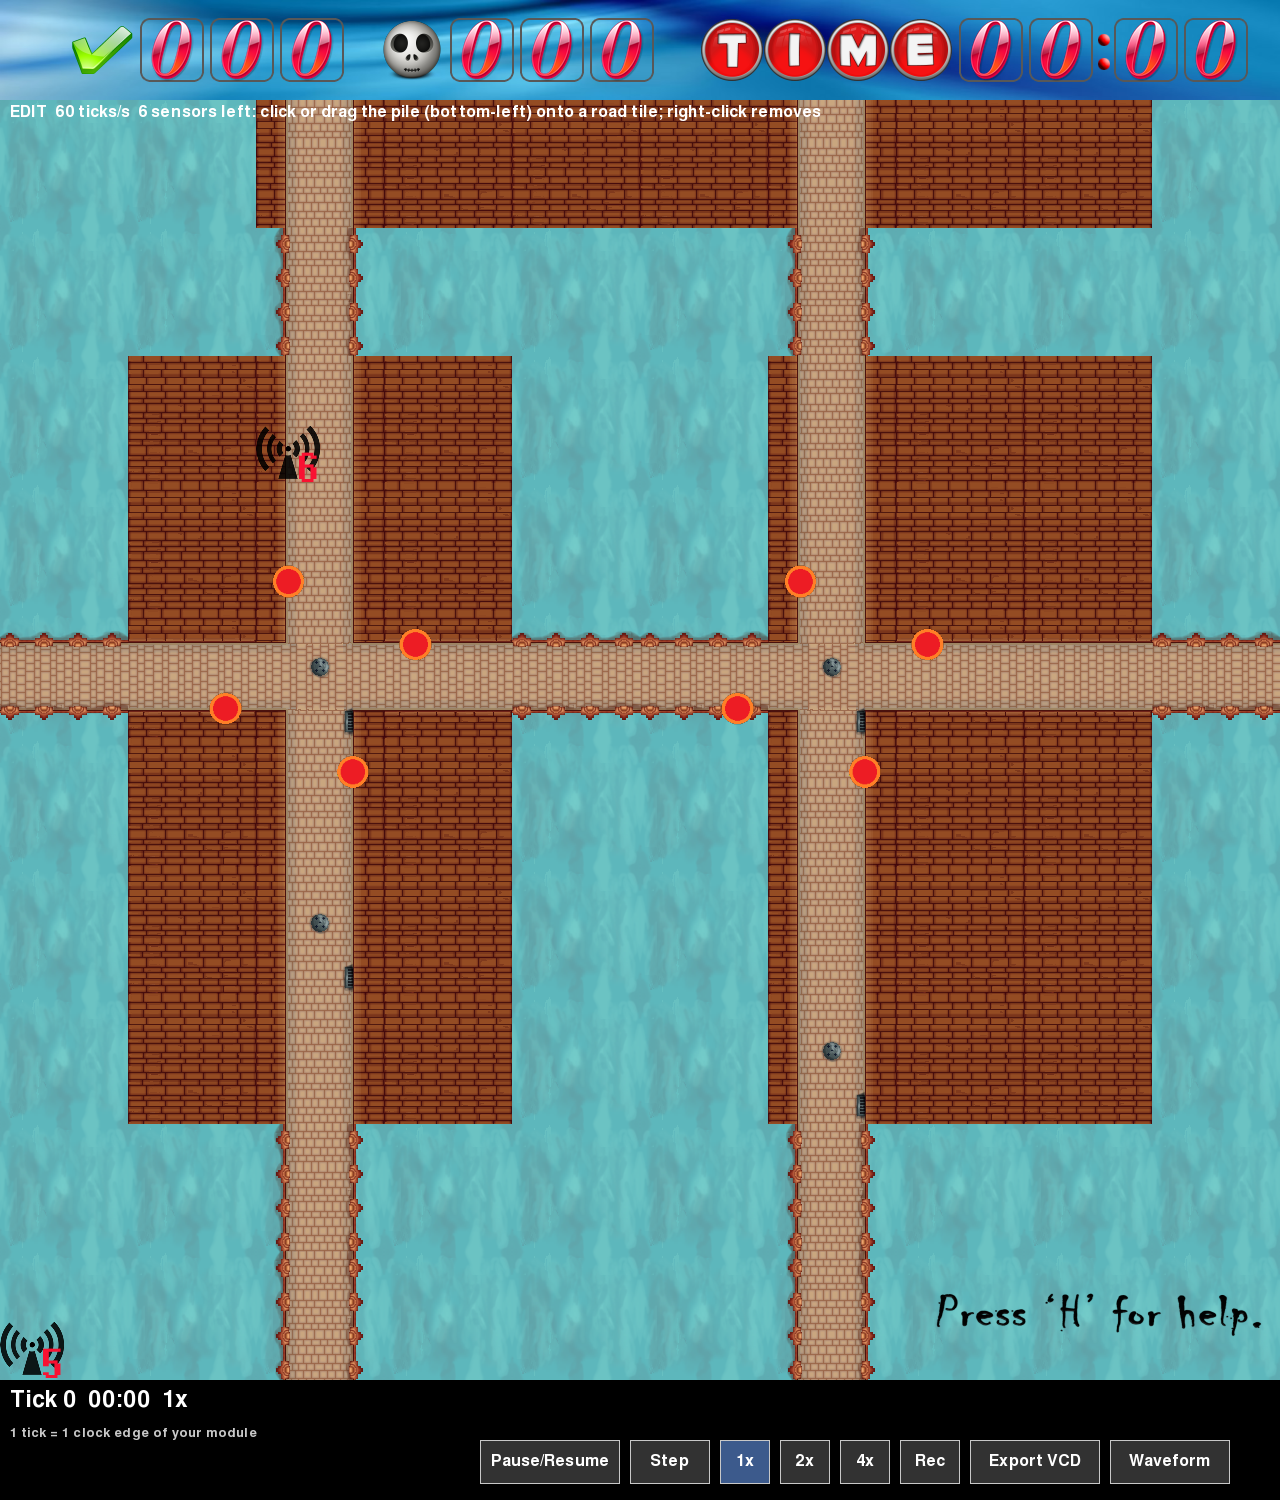
\includegraphics[width=0.46\linewidth]{images/gt-mg-drag.png}\hfill
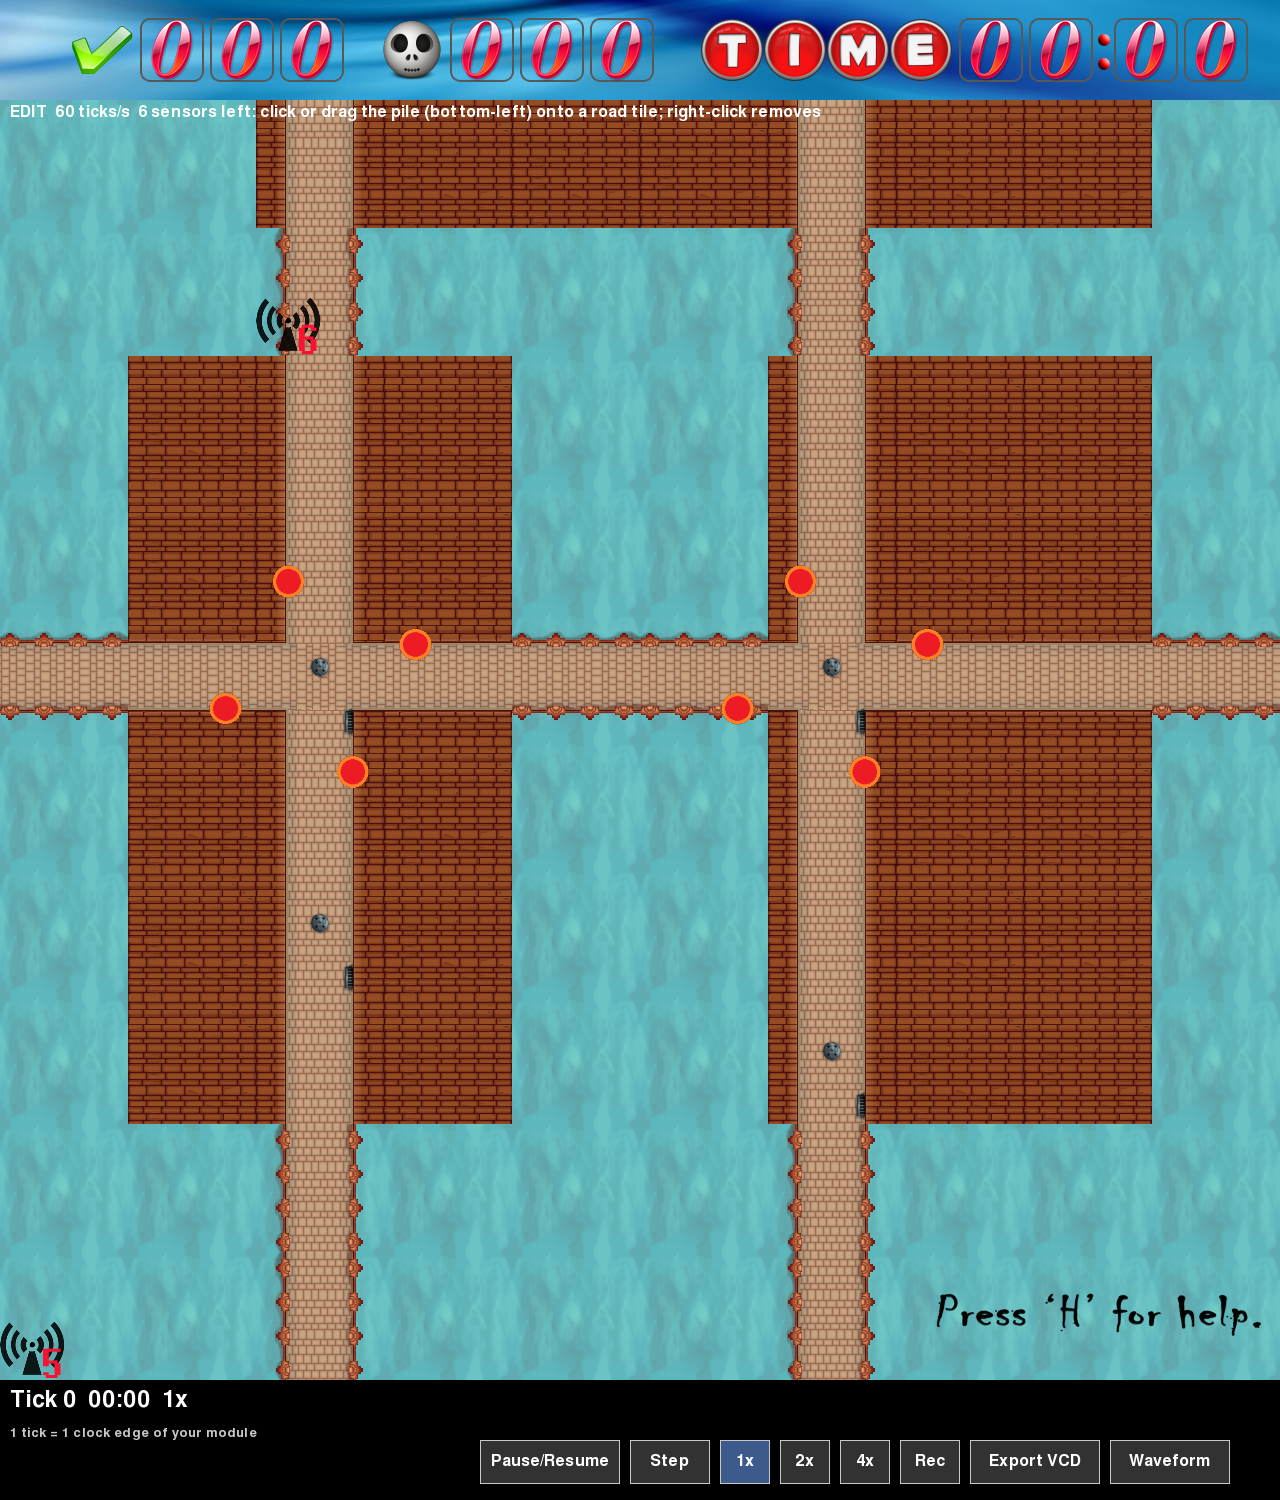
\includegraphics[width=0.46\linewidth]{images/gt-mg-dragged.png}
\caption{Dragging a placed sensor (left) and after releasing it on a new road tile (right).}\label{fig:gt-mg-drag}\label{fig:gt-mg-dragged}
\end{figure}

\subsubsection*{Writing the Verilog of a light}

Click an intersection: the Verilog editor opens with the file of that light (Figure~\ref{fig:gt-ve-open}). The module \cmd{light1} has the ports
\cmd{clk}, \cmd{rst} (active low), \cmd{sensor\_light} (8 bits: the entries and the inside of this intersection), \cmd{general\_sensors}
(30 bits: the sensors you placed), the four outputs \cmd{outN}, \cmd{outS}, \cmd{outE} and \cmd{outW} (3 bits: 0 Stop, 1 Forward only,
2 Left only, 3 Right only, 4 Go) and an optional \cmd{debug\_port}. Here the starter has one change, \cmd{assign debug\_port = general\_sensors;}, so the game
shows what the sensors deliver. Press \ui{Verify} to compile the file with Odin III (Figure~\ref{fig:gt-ve-verified}). Tick a box in the picture
of the intersection or type bits in \ui{Internal Sensors} and press \ui{Simulate} to step the module one cycle and print its outputs
(Figure~\ref{fig:gt-ve-simulated}): with a car on the north entry the light answers \cmd{OutN = 4}, Go. You can also edit the file in any editor; the game
notices the change and recompiles it in the edit phase.

\shot{gt-ve-open}{The Verilog editor with the file of the first light.}
\shot[0.9]{gt-ve-verified}{After \ui{Verify}.}
\shot[0.9]{gt-ve-simulated}{After \ui{Simulate} with a car on the north entry.}

\subsubsection*{Starting the simulation (S)}

Close the editor and press \ui{S}. The cars drive; the status line shows the speed and the tick rate, and the buttons under the map change
the speed, step, record, export a VCD and open a waveform. Press \ui{P} to pause when a car is on your sensor: the strip under the map then lists, for every
intersection, the inputs of the last tick and its four outputs (Figure~\ref{fig:gt-mg-run-paused}). Press \ui{S} to resume. When all cars are
done the score screen shows the cars that passed and the time in ticks (Figure~\ref{fig:gt-mg-score}); the ten best results of each level are kept.

\begin{figure}[H]\centering
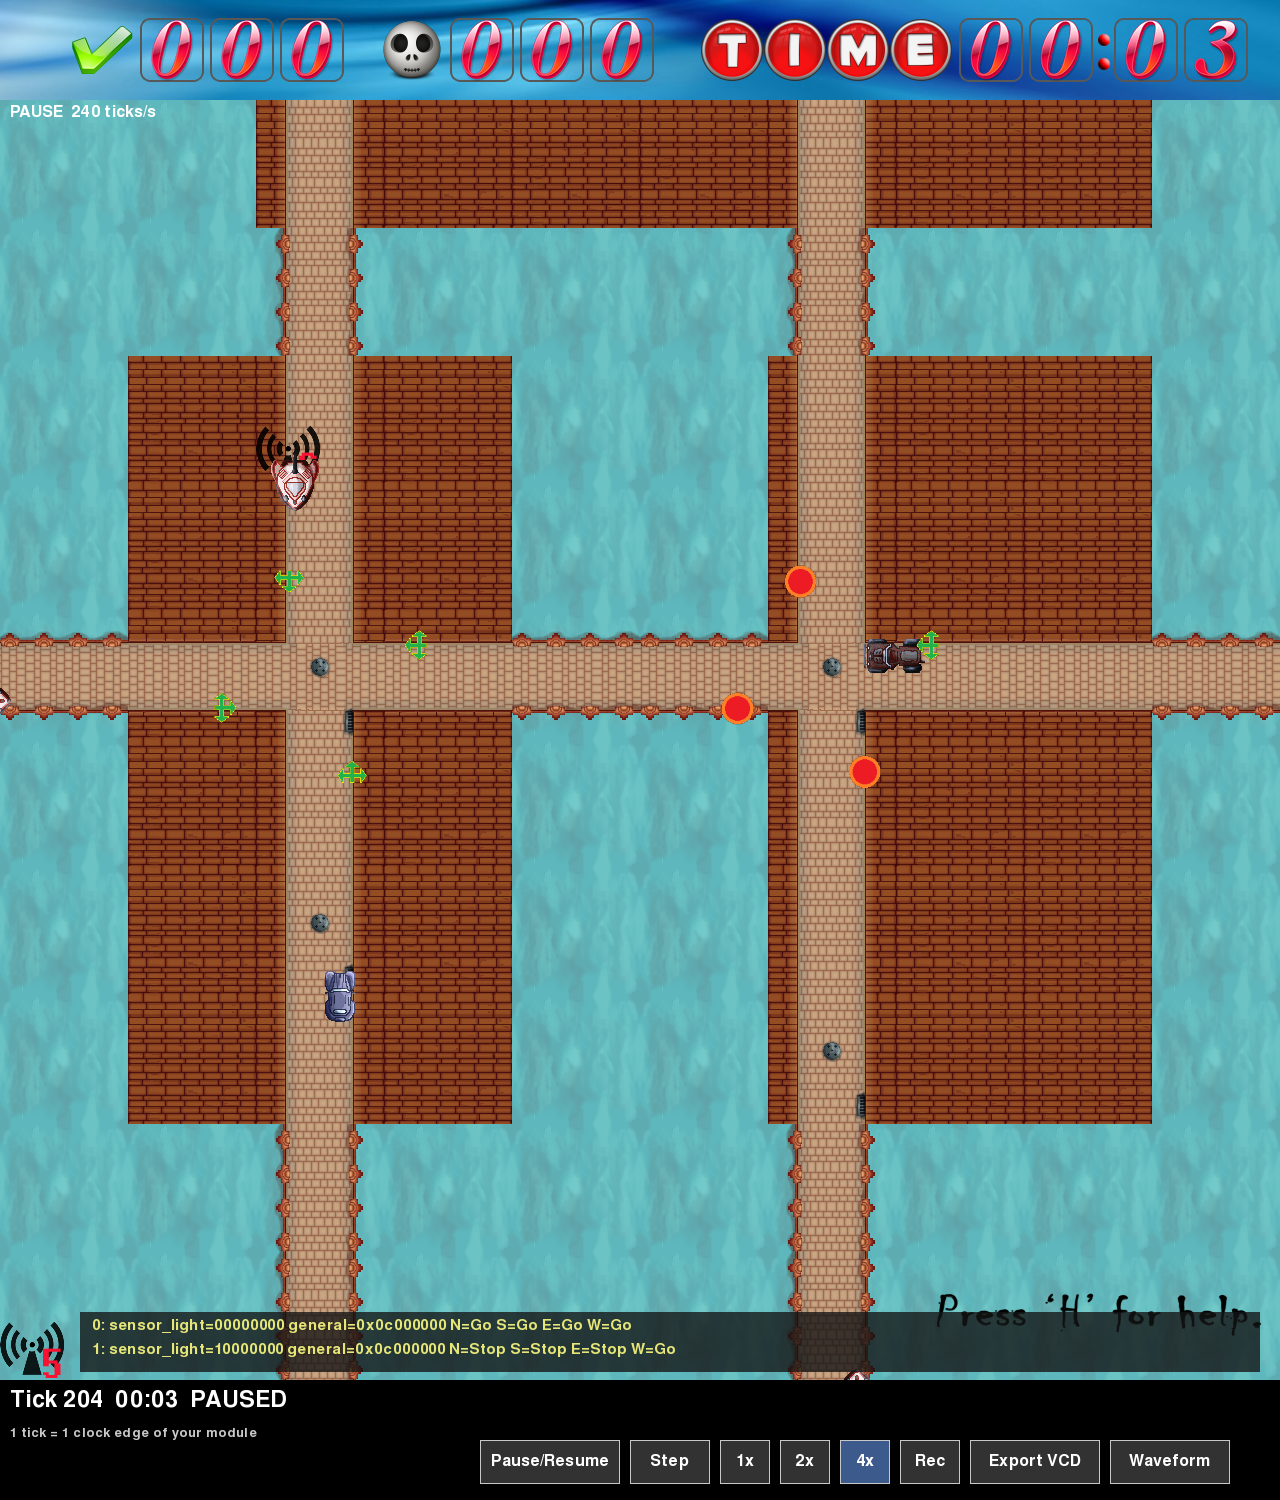
\includegraphics[width=0.46\linewidth]{images/gt-mg-run-paused.png}\hfill
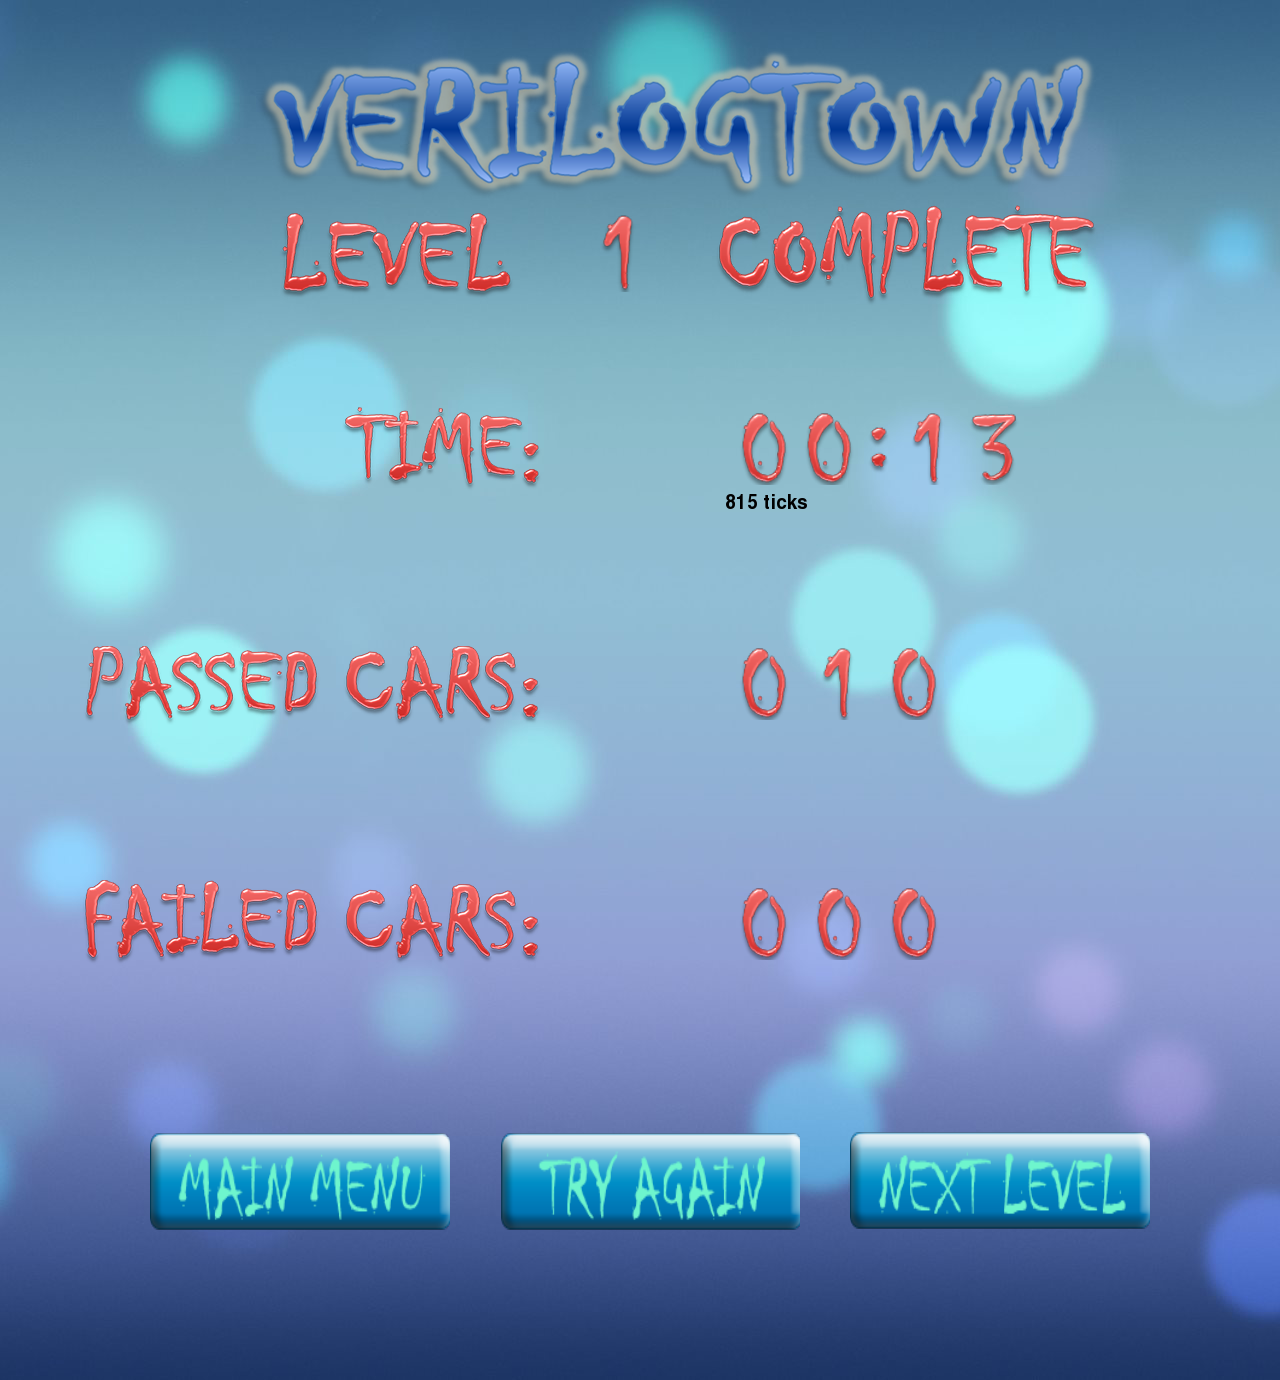
\includegraphics[width=0.46\linewidth]{images/gt-mg-score.png}
\caption{Level 1 paused with a car on the sensor (left) and the score screen (right).}\label{fig:gt-mg-run-paused}\label{fig:gt-mg-score}
\end{figure}

\subsubsection*{The level editor}

\menu{Tools \gt Midgard III Level Editor} opens a window for making your own levels (Figures~\ref{fig:gt-le-start} and~\ref{fig:gt-le-level1}); it needs no
pygame.

\shot[0.8]{gt-le-start}{The level editor start window.}
\shot[0.8]{gt-le-level1}{The level editor with level 1 loaded.}

\section{Where to Go Next}

\begin{itemize}
\item The Wyrd III manual: \url{https://drpaj12.github.io/wyrd/}, with every setting, option and key.
\item The command-line tutorial: \url{https://drpaj12.github.io/wyrd/wyrd-tutorial.pdf}, the same project run from a terminal, with the run
directory, \cmd{wyrd table}, \cmd{wyrd compare} and \cmd{wyrd sim}.
\item The Yggdrasil III hub, with the other tools of the suite (Odin III, Loki III) and how they fit together:
\url{https://github.com/drpaj12/YggdrasilIII}.
\end{itemize}

\end{document}
